% Compile de dentro de latex/, que é onde estão dispersao.pdf e
% referencias.bib:
%
%     latexmk -pdf slides.tex
%
% A saída é um PDF comum, uma página por passo de sobreposição.

\documentclass[aspectratio=169]{beamer}

\usepackage[T1]{fontenc}
\usepackage[brazilian]{babel}
\usepackage{amsmath}
\usepackage{booktabs}

% Temas distribuídos com a classe: default, Madrid, Berlin, Warsaw,
% metropolis (este último exige instalação à parte)
\usetheme{default}

% Sem isso, cada quadro traz uma barra de navegação que quase ninguém usa
\setbeamertemplate{navigation symbols}{}

\title{Ozônio e temperatura em Nova York}
\subtitle{Um exemplo de apresentação em Beamer}
\author{Fernando de Pol Mayer}
\institute{DEST/UFPR}
\date{\today}

\begin{document}

\frame{\titlepage}

\begin{frame}{O que vamos ver}
  \tableofcontents
\end{frame}

\section{Os dados}

\begin{frame}{Os dados}
  \begin{itemize}
    \item<1-> 153 observações diárias, de maio a setembro de 1973.
    \item<2-> Ozônio em ppb e temperatura em graus Fahrenheit.
    \item<3-> 37 dias sem medição de ozônio.
  \end{itemize}

  \vspace{0.5cm}
  \onslide<3->{Os valores faltantes não são aleatórios, e isso importa.}
\end{frame}

\begin{frame}{Médias mensais}
  \begin{table}
    \centering
    \begin{tabular}{lrr}
      \toprule
      Mês      & Ozônio (ppb) & Temperatura (F) \\
      \midrule
      Maio     & 23,6 & 65,5 \\
      Junho    & 29,4 & 79,1 \\
      Julho    & 59,1 & 83,9 \\
      Agosto   & 60,0 & 84,0 \\
      Setembro & 31,4 & 76,9 \\
      \bottomrule
    \end{tabular}
  \end{table}
\end{frame}

\section{O modelo}

\begin{frame}{O modelo}
  A regressão linear simples supõe
  \[
    Y_i = \beta_0 + \beta_1 x_i + \varepsilon_i,
    \qquad \varepsilon_i \sim \mathcal{N}(0, \sigma^2),
  \]
  e o estimador de mínimos quadrados é
  \[
    \hat{\boldsymbol{\beta}} =
    (\mathbf{X}^{\top}\mathbf{X})^{-1}\mathbf{X}^{\top}\mathbf{y}.
  \]

  \begin{block}{O que muda em relação ao artigo}
    Nada na matemática: os mesmos comandos, na mesma sintaxe.
  \end{block}
\end{frame}

\begin{frame}{Duas colunas}
  \begin{columns}[T]
    \column{0.48\textwidth}
    A relação é positiva, e a dispersão cresce com a temperatura.

    \vspace{0.3cm}
    \begin{itemize}
      \item Ajuste por mínimos quadrados.
      \item Variância não constante.
    \end{itemize}

    \column{0.48\textwidth}
    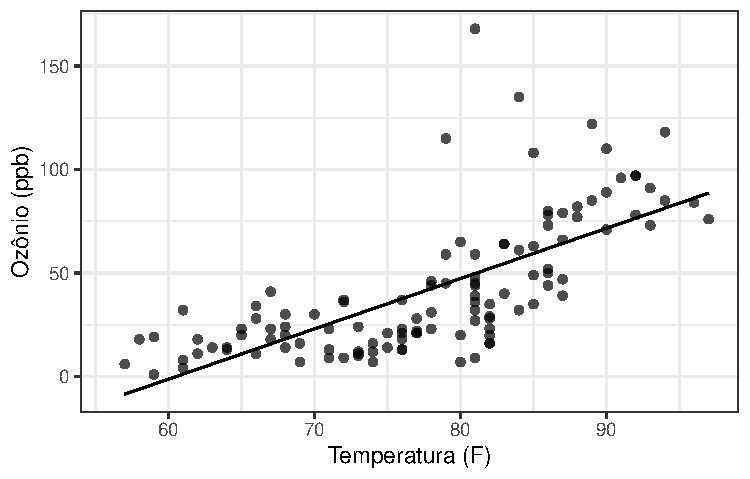
\includegraphics[width=\textwidth]{dispersao.pdf}
  \end{columns}
\end{frame}

\begin{frame}{Onde consultar}
  \begin{itemize}
    \item Lamport (1994), a referência da linguagem.
    \item Mittelbach e Fischer (2023), o \emph{Companion}.
    \item \url{https://ctan.org/}, os pacotes e a documentação de cada um.
  \end{itemize}

  \vspace{0.5cm}
  \centering
  \Large Obrigado.
\end{frame}

\end{document}
